\chapter{Distribución F}
Usada en teoría de probabilidad y estadística, la distribución F es una distribución de probabilidad continua. También se le conoce como distribución F de Snedecor (por George Snedecor) o como distribución F de Fisher-Snedecor (por Ronald Fisher).


\section{Descripción}
La distribución F es una distribución continua de muestreo de dos variables aleatorias independientes con distribuciones de chi-cuadrado, cada una de las cuales se divide entre sus grados de libertad. \cite{wiki:2}


En el caso de la binomial negativa, hallarémos la cantidad de \textit{n} primeros éxitos dentro de una serie de ensayos. Si fuese sólo el primer éxito, sería una geométrica.

\section{PDF}
\begin{center}
$\frac {\sqrt {\frac {(d_{1},x)^{d_{1}},d_{2}^{d_{2}}}{(d_{1}x+d_{2})^{d_{1}+d_{2}}}}} {x\,\mathrm {B} ({\frac {d_{1}}{2}},{\frac {d_{2}}{2}})}$
\end{center}
\subsection{Parámetros}
Los parámetros observables son:

\begin{center}
	\begin{tabular} {| l | l |}
		\hline
		$d_1$ & Grado de libertad\\ \hline
		$d_2$ & Grado de libertad\\ \hline		
	\end{tabular}
\end{center}

\section{CDF}
\begin{center}
	$I_{\frac{d_1 x}{d_1 x + d_2}}(d_1/2, d_2/2)\!$
\end{center}

\section{Media y Varianza}
\subsection{Media}
\begin{center}
$\mu = \frac{d_2}{d_2 - 2}$
\end{center}

\subsection{Varianza}
\begin{center}
	$\sigma^2 = {\frac {2\,d_{2}^{2}\,(d_{1}+d_{2}-2)}{d_{1}(d_{2}-2)^{2}(d_{2}-4)}}\!$
\end{center}
	
\section{MGF}
\begin{center}
	\textit{No definida}
\end{center}
	
\section{Gráficas}
\begin{center}
	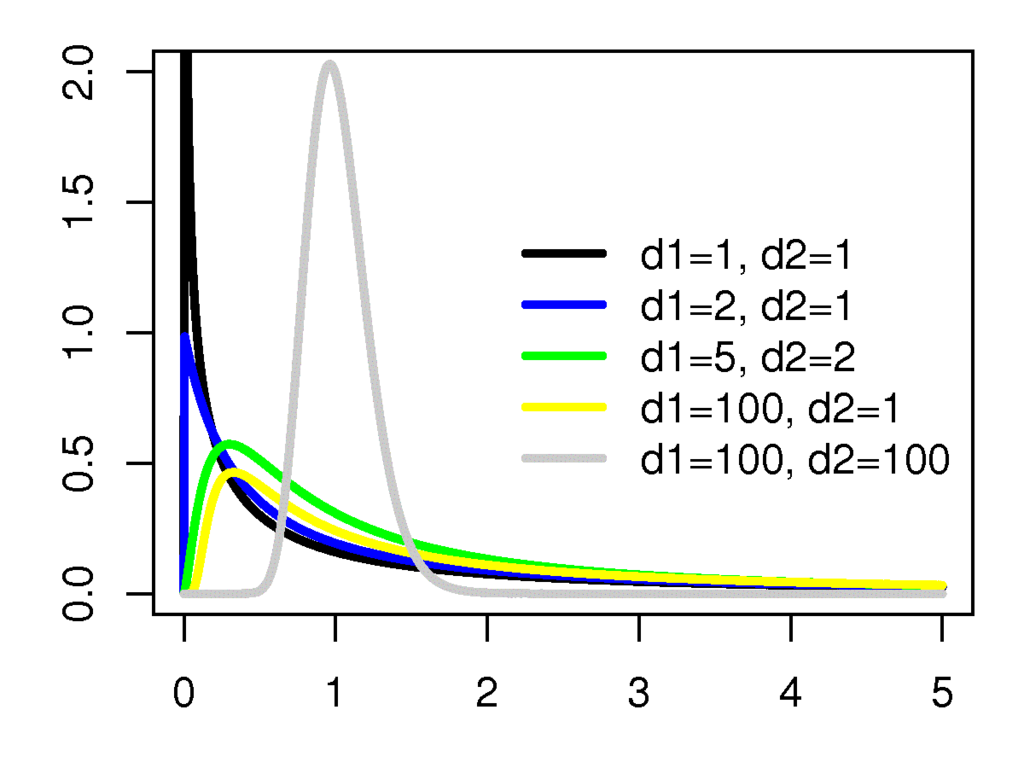
\includegraphics[scale=1.5]{imgs/f-pdf.png}
	
	\textit{PDF}
\end{center}

\begin{center}
	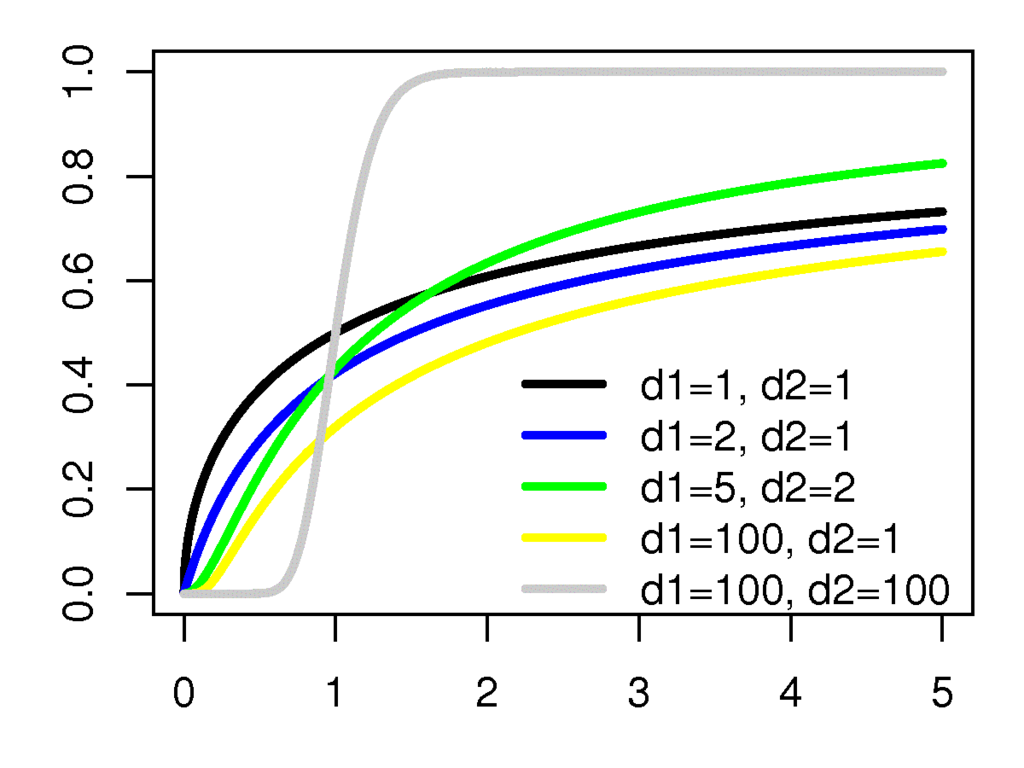
\includegraphics[scale=1.5]{imgs/f-cdf.png}
	
	\textit{CDF}
\end{center}

\section{Aplicaciones en la vida real}
La aplicación fundamental de la distribución F es la comparación de varianzas, es decir, el contraste de hipótesis referentes a varianzas de poblaciones normales e independientes, y a la comparación de medias de varias poblaciones, que constituye precisamente el “análisis de la varianza”.